%\documentclass[11pt]{exam}
\documentclass[11pt,answers]{exam}
\usepackage[headheight=1pt, includeheadfoot, headsep=1cm, top=1.5cm, bottom=1.3cm, left=2cm, right=2cm]{geometry}
\usepackage{mathtools}
\usepackage{amsmath,amsthm, amscd, amssymb, amsfonts}
\usepackage[english]{babel}
%\usepackage{fancyhdr}
\usepackage{enumitem}
\setlist{itemsep=0.5em}
\usepackage{xcolor}
\definecolor{forestgreen}{rgb}{0.13, 0.55, 0.13}
%\usepackage[colorlinks = true,
%linkcolor = forestgreen,
%urlcolor  = forestgreen,
%citecolor = forestgreen,
%anchorcolor = forestgreen]{hyperref}
\usepackage{multicol}
\usepackage{multienum}
\usepackage{euler}
\usepackage[OT1]{eulervm}
\renewcommand{\rmdefault}{pplx}
\usepackage{tikz}
\usepackage{mathabx}
\usepackage{lastpage}



\usepackage{tikz}
\usepackage{verbatim}
\usetikzlibrary{shapes.geometric,shapes.multipart,arrows,calc}


\pgfdeclarelayer{background}
\pgfdeclarelayer{foreground}
\pgfsetlayers{background,main,foreground}			
\tikzset{
	edge/.style = {black, ultra thick, outer sep=2pt},
	vertex/.style = {draw=black, very thick, fill=white, circle, minimum width=8pt, inner sep=2pt, outer sep=1pt},
	arc/.style = {black, ultra thick, outer sep=2pt, decoration={markings, mark=at position #1 with {\arrow[scale=1.5]{latex}}}, postaction=decorate},
	arc/.default = 0.58
}


%% header, footer definitions
\def\course{MATH 314}
\def\courselink{https://www.gsanmarco.com/graph-theory}
\def\assignment{Midterm Exam}
\def\assignlink{ds01.tex}
\def\due{March 9, 2023}


\lhead{\course}
\chead{\bfseries \assignment}
\rhead{\due}
\headrule



%\pagestyle{fancy}
%\fancyhead[L]{\course}
%\fancyhead[C]{\assignment} 
%\fancyhead[R]{\due} 
%\renewcommand{\footrulewidth}{0.4pt}
%\fancyfoot{}
%\fancyfoot[R]{\fontsize{8}{10} \selectfont  Page \thepage~of \pageref{LastPage}}
%\fancyfoot[L]{\fontsize{10}{12} \selectfont  Source file available at \href{\courselink}{\textbf{\courselink}}}

%% environments
% theorem style
\newtheorem{theorem}{Theorem}
\newtheorem{lemma}[theorem]{Lemma}
\newtheorem{corollary}[theorem]{Corollary}
\newtheorem{claim}[theorem]{Claim}
\newtheorem{defn}[theorem]{Definition}

% definition style
\theoremstyle{definition}
\newtheorem{problem}{Problem}
\newtheorem{Solution}{Solution}
% custom
%\newenvironment{solution}{\noindent\textbf{Solution.}}{\qed}

%% custom commands

\newcommand*{\abs}[1]{\lvert #1\rvert}     % absolute values, cardinality
\newcommand*{\eps}{\varepsilon}            % prettier epsilon
\newcommand*{\R}{\mathbb{R}}               % real numbers
\newcommand*{\C}{\mathbb{C}}               % complex numbers
\newcommand*{\Q}{\mathbb{Q}}               % rational numbers
\newcommand*{\Z}{\mathbb{Z}}               % integers
\newcommand*{\N}{\mathbb{N}}               % natural numbers
\newcommand*{\F}{\mathbb{F}}               % field
\newcommand*{\family}{\mathcal{F}}         % family
\newcommand*{\GL}{\mathbf{GL}}             % general linear group
\newcommand*{\what}[1]{\widehat{#1}}       % wider hat
\newcommand*{\wbar}[1]{\overline{#1}}      % wider bar
\newcommand*{\mcal}[1]{\mathcal{#1}}       % mathcal
\newcommand*{\mbf}[1]{\mathbf{#1}}         % mathbf
\newcommand*{\mbb}[1]{\mathbb{#1}}         % mathbb

% operators
\let\Pr\relax\DeclareMathOperator*{\Pr}{\mathbf{Pr}}       % probability
\DeclareMathOperator*{\E}{\mathbb{E}}          % expectation
\DeclareMathOperator*{\Var}{\mathbf{Var}}      % variance
\DeclareMathOperator*{\Span}{span}             % span
\DeclareMathOperator{\tr}{tr}                  % trace
\DeclareMathOperator{\rank}{rank}              % rank
\DeclareMathOperator{\supp}{supp}              % support
\DeclareMathOperator{\diam}{diam}



\begin{document}
\begin{center}
\parbox{5.5in}{\centering
				Name:\enspace\hrulefill.}
\end{center}

\noindent \textbf{Instructions} 
\begin{enumerate}[label*=$\bullet$, leftmargin=*, itemsep=.1em]
\item You may bring one standard 8.5x11 sheet of paper with handwritten notes.
\item Unless explicitly requested by a problem, do not include sketches as part of your proof.
%	\item In two questions, you will have the opportunity to choose between two options. 
\end{enumerate}

\addpoints
\begin{center}
	\gradetable[h][questions]
\end{center}
\hrulefill
\vskip10pt

\begin{questions}
	
	\question[25] 
Let $P=(u=v_0,v_1,\ldots,v_k=v)$, $k\geq 1$, be a $u$--$v$ geodesic in a connected graph $G$. 
Prove that $d(u,v_i)=i$ for each integer $i$ with $1\leq i\leq k$.
\begin{solution}
	Note for later use that $d(u,v)=k$, because $P=(u=v_0,v_1,\ldots,v_k=v)$ is a  geodesic.
	
	Fix any $i\in\{0,\dots,k\}$. Since$(u=v_0,v_1,\dots,v_i)$ is a $u$--$v_i$ path of length $i$, we know that $d(u,v_i)\leq i$. Suppose for the sake of contradiction that  $d(u,v_i)=\ell< i$; hence there is a $u$--$v_i$ geodesic $(u = w_0,\dots,w_\ell = v_i)$. But then $(u = w_0,\dots,w_\ell = v_i, v_{i+1},\dots,v_k= v)$ is a $u$--$v$ walk of length $\ell+(k-i)$.  Theorem 1.6 then implies that there is a $u$--$v$ path of length at most $\ell+(k-i)<k$, contradicting the previously established fact that $d(u, v) = k$.
\end{solution}


\question [25] 	Let $G$ be a connected graph and consider a function $f\colon V(G)\to X$ where $X$ is some arbitrary set.
	Prove that if $f$ is \emph{not} a constant function, then there is an edge $uv\in E(G)$ such that $f(u)\neq f(v)$. 
	
	Deduce that if $G$ is not regular, then $G$ contains adjacent vertices $u$ and $v$ such that $\deg u\neq\deg v$.


\begin{solution}
	Let us show the contrapositive statement. Thus we assume that for any pair of vertices $u, v$ in $G$, if $uv\in E(G)$ then $f(u)=f(v)$. To see that $f$ must be constant, fix any vertex $u^*$ in $G$. Now, for any other vertex $v$, since $G$ is connected, there is a $u^*$--$v$ path in $G$, say $(u^*=v_0, v_1, \dots, v_n=v)$. This means that $v_i v_{i+1} \in E(G)$ for each $i\in\{0, 1, \dots, n-1\}$, thus $f(v_i)=f(v_{i+1})$ for any such $i$. Putting these $n$ equations together, we get
	\[f(u^*)=f(v_0)=f(v_1)=f(v_2)=\dots=f(v_{n-1})=f(v_n)=f(v).\] 
	Thus $f(v)=f(u^*)$ for any $v\in V(G)$, and $f$ is constant. 
	
	In case $G$ is not regular, the degree function $\deg \colon V(G) \to \mathbb N$ is not constant. Hence we deduce from the statement above that there is an edge $uv\in E(G)$ such that $\deg u \ne \deg v$.
	\qed
\end{solution}



	\question[25] Apply both Kruskal's and Prim's Algorithms to find a minimum spanning tree in the following graph.
	In each case, show how this tree is constructed.
	\begin{center}
		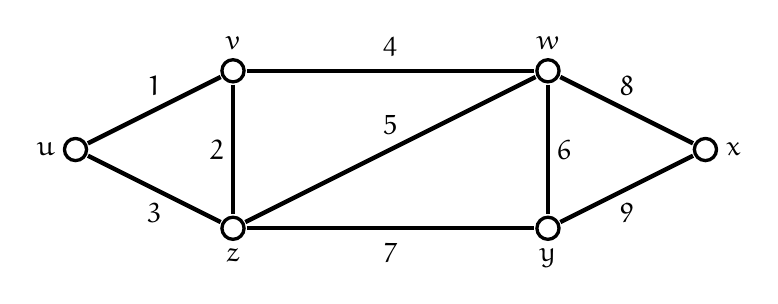
\begin{tikzpicture}[scale=1]
			\begin{pgfonlayer}{foreground}
				\node[vertex] (u) at (-4,0) {};
				\node[vertex] (z) at (-2,-1) {};
				\node[vertex] (v) at (-2,1) {};
				\node[vertex] (y) at (2,-1) {};
				\node[vertex] (w) at (2,1) {};
				\node[vertex] (x) at (4,0) {};
			\end{pgfonlayer}
			\begin{pgfonlayer}{main}
				\node[left,xshift=-4pt] at (u) {$u$};
				\node[below,yshift=-4pt] at (z) {$z$};
				\node[above,yshift=4pt]  at (v) {$v$};
				\node[below,yshift=-4pt] at (y) {$y$};
				\node[above,yshift=4pt]  at (w) {$w$};
				\node[right,xshift=4pt] at (x) {$x$};
			\end{pgfonlayer}
			\begin{pgfonlayer}{background}
				\draw[edge] (u) -- (v) node[midway,above] {$1$};
				\draw[edge] (u) -- (z) node[midway,below] {$3$};
				\draw[edge] (v) -- (z) node[midway,left,xshift=2pt] {$2$};
				\draw[edge] (v) -- (w) node[midway,above] {$4$};
				\draw[edge] (z) -- (y) node[midway,below] {$7$};
				\draw[edge] (z) -- (w) node[midway,above] {$5$};
				\draw[edge] (w) -- (y) node[midway,right,xshift=-2pt] {$6$};
				\draw[edge] (w) -- (x) node[midway,above] {$8$};
				\draw[edge] (y) -- (x) node[midway,below] {$9$};
			\end{pgfonlayer}
		\end{tikzpicture}
	\end{center}

\begin{solution}
	\begin{center}
	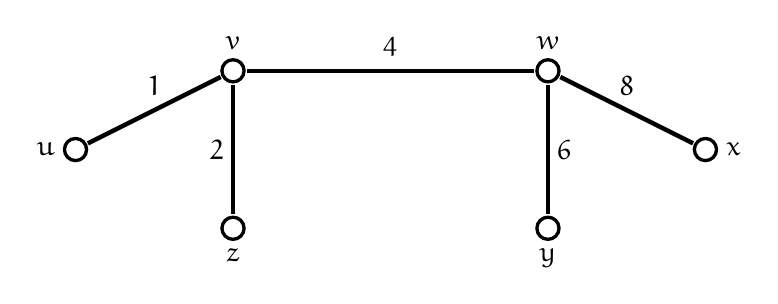
\begin{tikzpicture}[scale=1]
		\begin{pgfonlayer}{foreground}
			\node[vertex] (u) at (-4,0) {};
			\node[vertex] (z) at (-2,-1) {};
			\node[vertex] (v) at (-2,1) {};
			\node[vertex] (y) at (2,-1) {};
			\node[vertex] (w) at (2,1) {};
			\node[vertex] (x) at (4,0) {};
		\end{pgfonlayer}
		\begin{pgfonlayer}{main}
			\node[left,xshift=-4pt] at (u) {$u$};
			\node[below,yshift=-4pt] at (z) {$z$};
			\node[above,yshift=4pt]  at (v) {$v$};
			\node[below,yshift=-4pt] at (y) {$y$};
			\node[above,yshift=4pt]  at (w) {$w$};
			\node[right,xshift=4pt] at (x) {$x$};
		\end{pgfonlayer}
		\begin{pgfonlayer}{background}
			\draw[edge] (u) -- (v) node[midway,above] {$1$};
			%\draw[edge] (u) -- (z) node[midway,below] {$3$};
			\draw[edge] (v) -- (z) node[midway,left,xshift=2pt] {$2$};
			\draw[edge] (v) -- (w) node[midway,above] {$4$};
			%\draw[edge] (z) -- (y) node[midway,below] {$7$};
			%\draw[edge] (z) -- (w) node[midway,above] {$5$};
			\draw[edge] (w) -- (y) node[midway,right,xshift=-2pt] {$6$};
			\draw[edge] (w) -- (x) node[midway,above] {$8$};
			%\draw[edge] (y) -- (x) node[midway,below] {$9$};
		\end{pgfonlayer}
	\end{tikzpicture}
\end{center}
\end{solution}

	\question[25] 
	For this problem, you need to select \textbf{one of the two statements below}.

\begin{enumerate}[leftmargin=*, label=(\alph*)]
	\item Let $G$ be a self-complementary graph of order $n=4k$, where $k\geq 1$.
	Let $U=\{v : \deg v\leq n/2\}$ and $W=\{v : \deg v\geq n/2\}$.
	Prove that if $|U|=|W|$, then $G$ contains no vertex $v$ such that $\deg v=n/2$.
	
	\emph{Hint:} $\overline{G}$ contains at least $|W|$ many vertices with $\overline{G}$-degree strictly smaller than $n/2$.
	\item Prove that a $3$-regular graph $G$ has a cut-vertex if and only if $G$ has a bridge.
\end{enumerate}

\begin{solution}
\begin{enumerate}[leftmargin=*, label=(\alph*)]
\item Let $V=V(G)=V(\overline G)$. Recall that for any $v \in V$, we have $\deg_G v = n-1 - \deg_{\overline G} v$. 

Note that if $v \in W$, then $\deg_G v\geq n/2$, thus $\deg_{\overline G} v= n-1 - \deg_G v\leq n-1-n/2=n/2-1$. Hence $\overline{G}$ contains at least $|W|$ many vertices with $\overline{G}$-degree strictly smaller than $n/2$. 

Since $G \cong \overline G$, we deduce that also $G$ contains $|W|$ many vertices with $G$-degree strictly smaller than $n/2$. Since $|W| = |U| = |\{ v : \deg v\leq n/2 \} |$, this means that any vertex $v$ in $U$ must satisfy $\deg_G v <n/2$. Hence  $G$ contains no vertices of degree $n/2$.

\item Since a graph is $3$-regular if and only if all its components are $3$-regular, by reducing the argument to a component, we can assume that $G$ is connected.

Assume first $G$ has a bridge $e=uv$. Then, by Theorem 5.1, $u$ and $v$ are cut vertices, because both have degree $\geq 2$.

Conversely, let $v$ be a cut-vertex. Since $v$ has exactly $3$ neighbors, $G-v$ has either $2$ or $3$ components. If $G-v$ has $2$ components one of these has two neighbors and the other has one. If $G-v$ has $3$ components, then each of these contains only one neighbor. In either case, we see that there is a component $H$ of $G-v$ with exactly one neighbor of $v$, which we denote by $u$. 

We show that $e=uv$ is a bridge of $G$. Indeed, we show that $e$ is the unique $u$--$v$ path in $G$. For a contradiction, if $(u=v_0, v_1, \dots, v_n=v)$ is a $u$--$v$ path in $G$ of length $n\geq 2$, then the vertices $v_1, \dots, v_{n-1}$ must be in $V(H)$, since they connect to $u=v_0$ without passing trough $v=v_n$. But then $v_{n-1}$ is a vertex in $H$ such that $v_{n-1} v$ is an edge in $G$, which contradicts that $u$ is the unique $G$-neighbor of $v$ in $H$. Hence $e$ is a bridge. 

\textbf{Note:} it is not true that two incident cut-vertices form a bridge.
\end{enumerate}
\end{solution}
\end{questions}

\end{document}


